\chapter{Modelagem do sistema: 360 video streaming}\label{Cap:Problem Design}
\section{O vídeo esférico}

O video esférico, diferente do vídeo tradicional plano, é um tipo de vídeo que pode ser projetado na casca interna de uma esfera, onde o usuário, localizado no centro, possui três graus de liberdade para olhar ao redor movimentando a cabeça. A captura do vídeo começa em um arranjo de câmeras tradicionais que captura o ambiente ao redor. As várias imagens das câmeras são sincronizadas e costuradas em uma esfera formando uma única imagem. Para utilizar os codificadores de vídeo populares como HEVC, AV1, VP9, etc, o vídeo precisa ser mapeado em um plano através de técnicas de projeção cartográficas, como a projeção equirretangular (ERP) e projeção cubemap (CMP) para ser comprimido, encapsulados em arquivos MP4, por exemplo e armazenados ou transmitidos pela rede. Desta forma, para poder manipular os pixels no domínio da projeção e da esfera, extrair o viewport e calcular a qualidade do vídeo, foi necessário desenvolver uma nova biblioteca que realize o mapeamento ente diferentes sistemas coordenadas para as projeções equirretangular e cubemap. Para isto foi definido a relação entre os sistemas de coordenadas cartesiano, horizontal e sistema de coordenadas de corpo conforme descrito a seguir.

\subsection{Os Sistemas de Coordenadas}

O sistema de coordenadas cartesiano, dextrógiro, representado na figura~\ref{fig:coordenadas} é usado para descrever e operar a esfera no espaço de 3 dimensões através de operações de álgebra linear. O vídeo esférico é representado com o usuário no centro de uma esfera de raio 1. Na posição inicial, o eixo Z aponta para a frente, o eixo X aponta para a direita e o eixo Y aponta para baixo. Como o campo de visão do usuário é limitado pelo sistema visual humano, ele visualiza apenas uma parte da esfera, chamada de Viewport.

\begin{figure}[htbp]
\centering

\subfigure[Sistema de coordenadas de referência em um espaço cartesiano. \label{fig:coordenadas}]
    {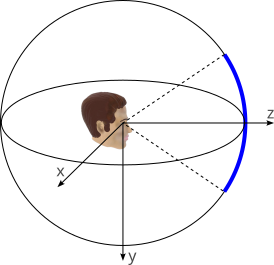
\includegraphics[width=0.25\linewidth]{fig/coordenadas.png}} \quad
\subfigure[Sistema de coordenadas horizontal em um espaço cartesiano. \label{fig:hcs}]
    {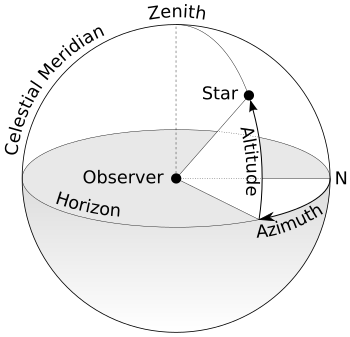
\includegraphics[width=0.25\linewidth]{fig/hcs.png}} \quad
\subfigure[Sistema de coordenadas de corpo em um espaço cartesiano. \label{fig:bcs}]
    {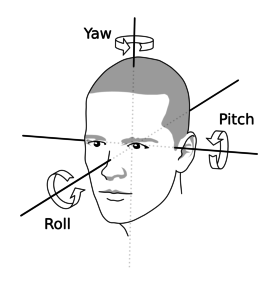
\includegraphics[width=0.25\linewidth]{fig/bcs.png}} \quad

\caption{Os Sistemas de Coordenadas}
\label{fig:coord_sis}
\end{figure}

% \subsubsection{Sistema Horizontal}
Para representar um ponto na esfera do vídeo, uma variação do sistema de coordenadas esféricas, chamado de sistema de coordenadas horizontal é usado como intermediário para operações entre projeções. O sistema de coordenadas horizontal, muito usado na astronomia para observação de corpos celestes, utiliza ângulos para representar a posição dos pixels na esfera do vídeo. Como mostra a figura~\ref{fig:hcs}, neste sistema, as coordenadas são relativas ao horizonte (plano ZX) e a posição inicial, isto é, o eixo Z positivo. 

A elevação varia de -90° a 90°, sendo que o sinal positivo aponta para acima do horizonte, enquanto que o azimute varia de -180° a 180°, sendo que o sinal positivo está à direita do eixo Z. Desta forma, o pixel na posição (elevação, azimute) igual a (0,0) encontra-se no ponto (x=0, y=0, z=1). As equações para conversão das coordenadas cartesianas em coordenadas horizontais são:

\begin{align}
    r &= \sqrt{x^2+y^2+z^2} \\
    \text{Azimute} &=\sin^{-1}\left(\frac{-y}{r}\right) \\
    \text{Elevação} &=\tan^{-1}\left(\frac{x}{z}\right)\\
    \label{eq:cart2hcs}
\end{align}

% \subsubsection{Coordenadas de Corpo}

O sistema de coordenadas de corpo, também usado para modelagem de aeronaves é usado para modelar o movimento da cabeça do usuário e sua orientação coincide com o sistema de coordenadas horizontal. Este sistema consiste de ângulos relativos à posição inicial (elevação=0 e azimute=0 no sistema horizontal, ou o vetor (0, 0, 1) no sistema cartesiano) e é usado para representar o movimento da cabeça do usuário usando ângulos de Euler, como mostra a figura~\ref{fig:bcs}. por se tratar de rotação, os valores dos ângulos podem assumir qualquer valor (em radianos).

Assim, rodar o usuário em uma direção é equivalente a rodar a esfera na direção oposta. O movimento de \textit{pitch} é realizado olhando em direção ao eixo X e rodando a esfera. O movimento de \textit{yaw} é realizado rodando a esfera em relação ao eixo Y e o \textit{roll} é realizado rodando a esfera em relação ao eixo Z. É convencionado que todas as rotações em sentido horário são positivas e em sentido anti-horário são negativas. Assim, olhar para cima possui um \textit{pitch} positivo, olhar para a direita possui um yaw positivo e rodar a cabeça em sentido horário possui um ângulo \textit{roll} positivo.

A nova posição dos pixels na posição (x’, y’, z’) da esfera é dada pelo produto matricial da posição dos pixels por uma matriz de rotação R, conforme equação abaixo.

\begin{align*}
    \begin{bmatrix}
        X\\
        Y\\
        Z
    \end{bmatrix}
    =
    R \times
    \begin{bmatrix}
        X'\\
        Y'\\
        Z'
    \end{bmatrix}
\end{align*}

A matriz de rotação para os ângulos (yaw, pitch, roll) é dada pelo produto matricial das matrizes de rotação do eixo X, Y e Z na seguinte ordem:

\begin{align*}
R=Y\times X\times Z
\end{align*}

As matrizes individuais são:

\begin{align*}
R_X &=\begin{bmatrix}
1 & 0 & s0\\
0 & cos(pitch) & -sin(pitch)\\
0 & sin(pitch) & cos(pitch)
\end{bmatrix}
\\
R_Y &=\begin{bmatrix}
cos(yaw) & 0 & sin(yaw)\\
0 & 1 & 0\\
-sin(yaw) & 0 & cos(yaw)
\end{bmatrix}
\\
R_Z &=\begin{bmatrix}
cos(roll) & -sin(roll) & 0\\
sin(roll) & cos(roll) & 0\\
0 & 0 & 1
\end{bmatrix}
\end{align*}


\subsection{Projeções}

\subsubsection{Projeção Equirretangular}

A projeção equirretangular é uma técnica de mapeamento cartográfico de uma esfera para um plano retangular, preservando a proporção dos elementos na imagem, ou seja, os pixels na imagem mapeada têm uma relação de aspecto constante. Isso significa que a imagem resultante tem a mesma largura para altura em todos os pontos, o que simplifica sua representação digital e facilita o processo de visualização em plataformas de vídeo e dispositivos, como mostra a figura~\ref{fig:erp}.


\begin{figure}
    \centering
    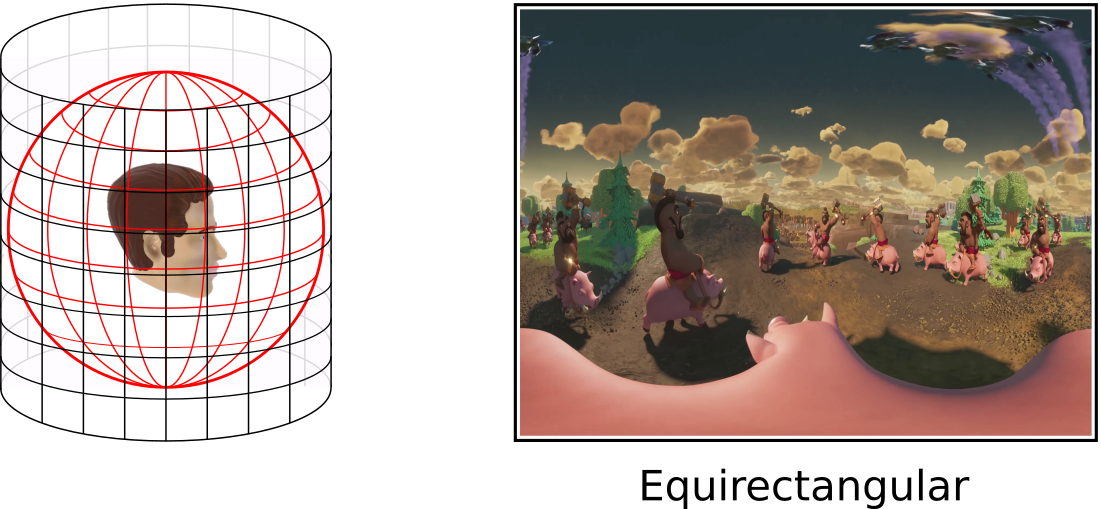
\includegraphics[width=0.8\textwidth]{fig/erp.png}
    \caption{Projeção Equirretangular mapeada no plano da imagem.}
    \label{fig:erp}
\end{figure}

No mapeamento de um vídeo 360° usando a projeção equirretangular, a esfera do vídeo é desdobrada em um plano 2D retangular, onde cada ponto na esfera é mapeado para um ponto correspondente na imagem retangular. Primeiro, a posição do pixel na esfera em coordenadas cartesianas é convertido para o sistema de coordenadas horizontal usando as equações~\ref{eq:cart2hcs}. Em seguida, as coordenadas são normalizadas em um plano uv onde u e v variam de 0 a 1, o eixo u aponta para a direita e o eixo v aponta para baixo usando as equações~\ref{eq:hcs2erp}. Por fim as coordenadas $(m, n)$ na imagem são dadas multiplicando $u$ e $v$ pela largura ($W$) e altura ($H$) da  imagem, respectivamente. O truncamento é realizado afim de se aplicar a interpolação por vizinho mais próximo.

\begin{align}
    u &= \dfrac{\text{Azimute}}{2\pi} + 0.5 \\
    v &= \dfrac{-\text{Elevação}}{\pi} + 0.5 \\
    \label{eq:hcs2erp}
\end{align}

\subsubsection{Projeção Cubemap}

A projeção cubemap é outra técnica comumente usada em vídeos 360° para mapear um ambiente tridimensional em uma representação bidimensional, atualmente adotado pelo Youtube e pelo Facebook. Ao contrário da projeção equirretangular, que mapeia a esfera em um plano retangular, a projeção cubemap mapeia a esfera em seis faces quadradas de um cubo de lado igual a 2. As seis faces correspondem a visão ao redor do ponto de captura. As faces geralmente são organizadas em uma grade de 3x2 formando um único arquivo de imagem. As três imagens superiores são as faces da esquerda, frente e direita, Enquanto as faces de baixo são rotacionadas 90° em sentido horário e correspondem as faces de cima, de trás e de baixo. A figura~\ref{fig:cmp} mostra um exemplo de mapeamento para projeção Cubemap (CMP).

\begin{figure}
    \centering
    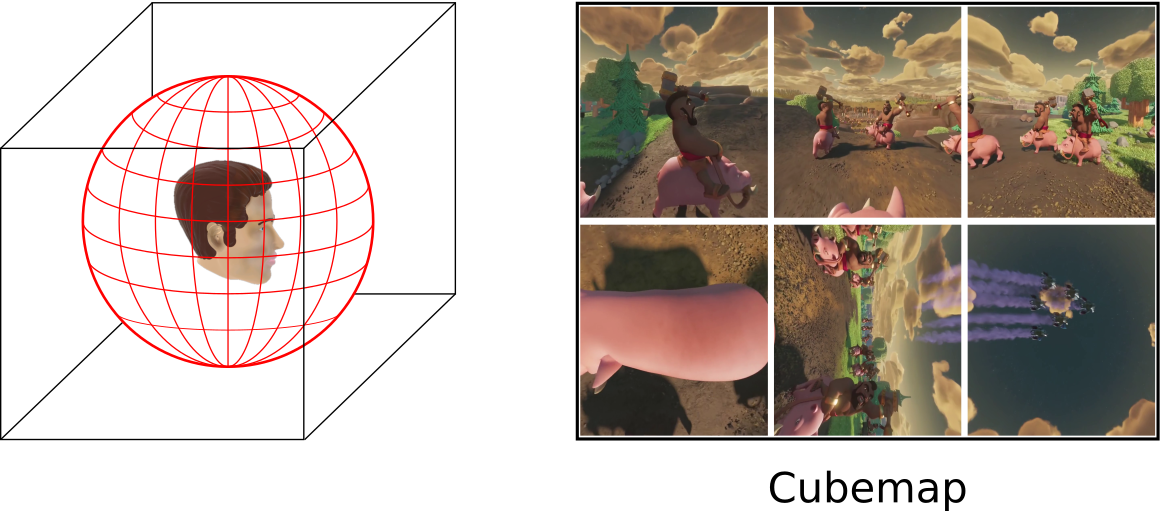
\includegraphics[width=0.8\textwidth]{fig/cmp.png}
    \caption{Projeção Cubemap e a disposição das seis faces no plano da imagem.}
    \label{fig:cmp}
\end{figure}

Como forma de representação auxiliar, cada face é mapeada em um plano $uv$ conforme a tabela~\ref{tab:uv_erp}, onde as coordenadas $u$ e $v$ variam de -1 a +1, com $u$ apontando para direita e $v$ apontando para baixo. Por fim, as coordenadas $uv$ são convertidas para posições dos pixels pela equação $ (uv+1)\times \frac{A}{2}-0.5$, onde A é o número de pixels em uma face do quadrado, e reposicionado na imagem. O processo inverso, de mapeamento do plano uv para o espaço cartesiano é feito pela tabela~\ref{tab:uv_erp}.

\begin{table}[htbp]
    \centering
    \caption{Tabela de coordenadas $(X, Y, Z)$ em função de $(U, V)$}
    \label{tab:uv_erp}
    \begin{tabular}{|c|c|c|c|}
    \hline
    \textbf{Face} & \textbf{X} & \textbf{Y} & \textbf{Z} \\
    \hline
    0 & $-1.0$ & $v$    & $u$    \\
    1 & $u$    & $v$    & $1.0$  \\
    2 & $1.0$  & $v$    & $-u$   \\
    3 & $-u$   & $1.0$  & $v$    \\
    4 & $-u$   & $v$    & $-1.0$ \\
    5 & $-u$   & $-1.0$ & $-v$   \\
    \hline
    \end{tabular}
\end{table}

\begin{table}[htbp]
    \centering
    \caption{Tabela de condições e valores de \( face, u, v \) em função de $(X, Y, V)$}
    \label{tab:condicoes}
    \begin{tabular}{|c|c|c|c|}
    \hline
    \textbf{Condição} & \textbf{Face} & \textbf{u} & \textbf{v} \\
    \hline
    $ |X| \geq |Z|  \text{ e }  |X| \geq |Y|  \text{ e }  X < 0 $ & 0 &  $\frac{Z}{|X|}$ & $ \frac{Y}{|X|} $ \\
    $ |Z| \geq |X|  \text{ e }  |Z| \geq |Y|  \text{ e }  Z > 0 $ & 1 &  $\frac{X}{|Z|}$ & $ \frac{Y}{|Z|} $ \\
    $ |X| \geq |Z|  \text{ e }  |X| \geq |Y|  \text{ e }  X > 0 $ & 2 &  $\frac{-Z}{|X|}$  & $ \frac{Y}{|X|} $ \\
    $ |Y| \geq |X|  \text{ e }  |Y| \geq |Z|  \text{ e }  Y < 0 $ & 3 &  $\frac{-X}{|Y|} $ & $ \frac{Z}{|Y|} $ \\
    $ |Z| \geq |X|  \text{ e }  |Z| \geq |Y|  \text{ e }  Z < 0 $ & 4 &  $\frac{-X}{|Z|}$  & $ \frac{Y}{|Z|} $ \\
    $ |Y| \geq |X|  \text{ e }  |Y| \geq |Z|  \text{ e }  Y > 0 $ & 5 &  $\frac{-X}{|Y|}$  & $ \frac{-Z}{|Y|} $ \\
    \hline
    \end{tabular}
\end{table}

\subsection{O Viewport}

O viewport é definido como a porção da esfera que é visível pelo usuário. Como a visão humano (FOV -\textit{ Field of View}) é limitada, os HMD reproduzem um FOV de aproximadamente $120^\circ\times90^\circ$. Para isto os ponto da esfera que pertencem ao viewport são projetados a um plano tangente a esfera no ponto $ P(0, 0, 1) $ utilizando a projeção Gnomônica ou Retilínea\footnote{https://www.wolframalpha.com/input?i=rectilinear+projection}, como pode ser visto na figura~\ref{fig:projecao_viewport}. 

\begin{figure}[htb]
    \centering
    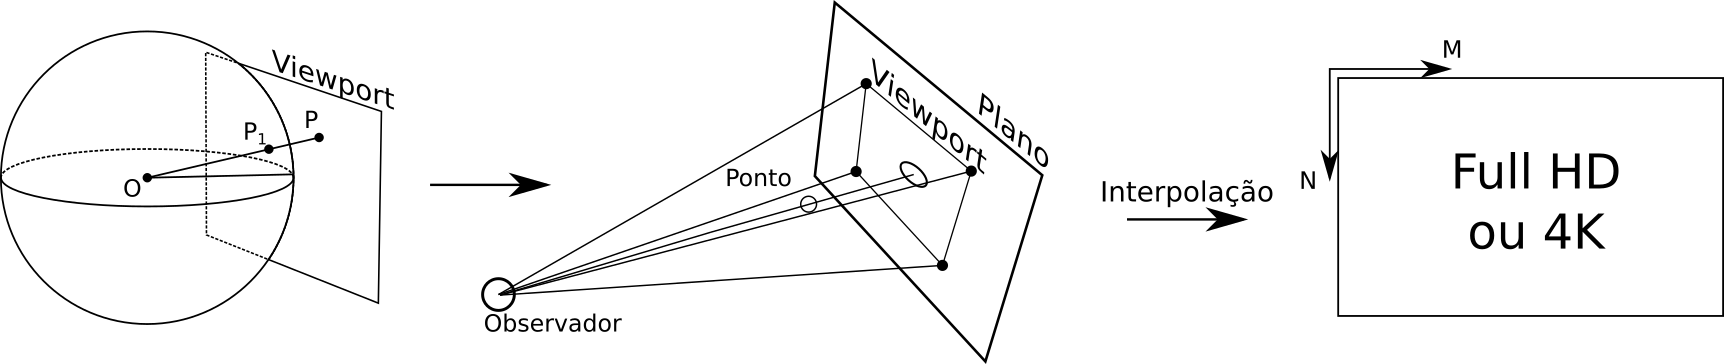
\includegraphics[width=1.0\linewidth]{fig/projecao_viewport.png}
    \caption{Extração do viewport usando projeção retilinear ou gnomônica.}
    \label{fig:projecao_viewport}
\end{figure}

Primeiramente, a matriz da imagem do viewport é pre alocada de acordo com a resolução exibida para o usuário. Em vez do valor do pixel, cada célula da matriz é preenchida com a posição do pixel na esfera usando coordenadas horizontais, de $-fov_X$ a $+fov_X$ e de $-fov_Y$ a $+fov_y$. Em seguida, cada coordenada é convertida para o sistema cartesiano usando as equações~\ref{eq:cart2hcs}. Finalmente as coordenadas cartesianas são convertidas para o domínio da projeção, seja equirretangular ou cubemap. Obviamente os pontos não serão os mesmos, então é usado algum método de interpolação, com interpolação por vizinho mais próximo ou interpolação linear. Agora basta mapear os pixels do viewport com os pixels da projeção.

Por outro lado, para verificar quais ladrilhos pertencem ao viewport, é preciso verificar se um pixel da projeção está sendo visualizado. Para isto, consideramos que o viewport compreende o espaço interno da intersecção de quatro planos que passam pelo centro da esfera e possuem inclinação relativas ao FOV do viewport e ao eixo Z. Por exemplo, um FOV de $ 120^\circ\times 90^\circ $ está limitado a 60° à direita e -60° à esquerda do eixo Z e 45° acima e -45° abaixo do eixo Z. Estes planos definem os limites superiores, inferiores, esquerdo e direito do viewport. Estas normais devem apontar para o lado de fora do viewport, assim o viewport compreende apenas os pontos que estão abaixo de todos os planos ao mesmo tempo. As normais que definem os planos são descritas na equação~\ref{eq:normals}, onde $fov_X$ e $fov_Y$ são os ângulos horizontal e vertical do FOV, respectivamente.

\begin{align}
N &=\begin{bmatrix}
     0 & -cos\left(\dfrac{fov_Y}{2}\right) & -sin\left(\dfrac{fov_Y}{2}\right) \\
     0 & sin\left(\dfrac{fov_Y}{2}\right) & -cos\left(\dfrac{fov_Y}{2}\right) \\
     cos\left(\dfrac{fov_X}{2}\right) & 0 & -sin\left(\dfrac{fov_X}{2}\right)\\
     -sin\left(\dfrac{fov_X}{2}\right) & 0 & -cos\left(\dfrac{fov_X}{2}\right)
\end{bmatrix}
\label{eq:normals}
\end{align}

Após o movimento de cabeça, as normais são rotacionadas de acordo com as coordenadas de corpo $H(yaw, pitch, roll)$ e assumem nova posição $ N_R $ dado pelo produto matricial do vetor de normais com a matriz de rotação $ N_R = \textbf{N} \times \textbf{R}$. Um pixel $ \textbf{P}$ qualquer no espaço cartesiano pertencerá ao viewport se o produto interno $ N.T \dot P <=0 $ para todas as normais, ou seja, estão abaixo das normais após as normais forem rotacionadas durante o movimento da cabeça.

\section{Qualidade objetiva do vídeo}

\subsection{Qualidade para o cliente}
No processo de preparação para o \textit{streaming} de vídeos esféricos, a esfera de vídeo passa por um mapeamento em um plano, introduzindo distorções que variam ao longo do plano. Ao utilizar métodos de compressão com perda, os codificadores geralmente aplicam a quantização de forma uniforme em todo o quadro, podendo impactar mais severamente em regiões distorcidas pela projeção. Após a decodificação, os pixels renderizados são remapeados de volta para a esfera, e quaisquer artefatos de codificação, como blocados, aliasing, efeito de \textit{Gibbs}, borrado, etc, também serão distorcidos.

Assim, a qualidade objetiva da viewport é definida como a disparidade entre o viewport extraído do vídeo codificado e o viewport de um vídeo de referência.   A Figura~\ref{fig:QualityWorkflow} ilustra como medir a qualidade objetiva do \textit{viewport}, considerando a esfera sem degradação e a esfera recuperada após a compressão. A viewport precisa ser extraída com base na posição da cabeça do usuário em ambos os vídeos de referência e codificado, assim o MSE e SSIM devem ser calculados entre esses quadros. O MSE foi usado no lugar do PSNR, pois o PSNR deve ser calculado apenas após o cálculo da média do MSE de todos os quadros de um vídeo, como mostra a documentação do filtro de PSNR do ffmpeg\footnote{https://ffmpeg.org/ffmpeg-filters.html}. As operações de cálculo MSE e do SSIM foram calculadas usando a biblioteca scikit-image. Apesar do MSE e o SSIM falhem ao tentar medir qualidade sob certas condições, elas são suficientes para se medir distorções produzidas por artefatos esperados como bordas de ladrilho, borrado e blocado.~\cite{Bovik2009} 

\begin{figure}[ht]
    \centering
    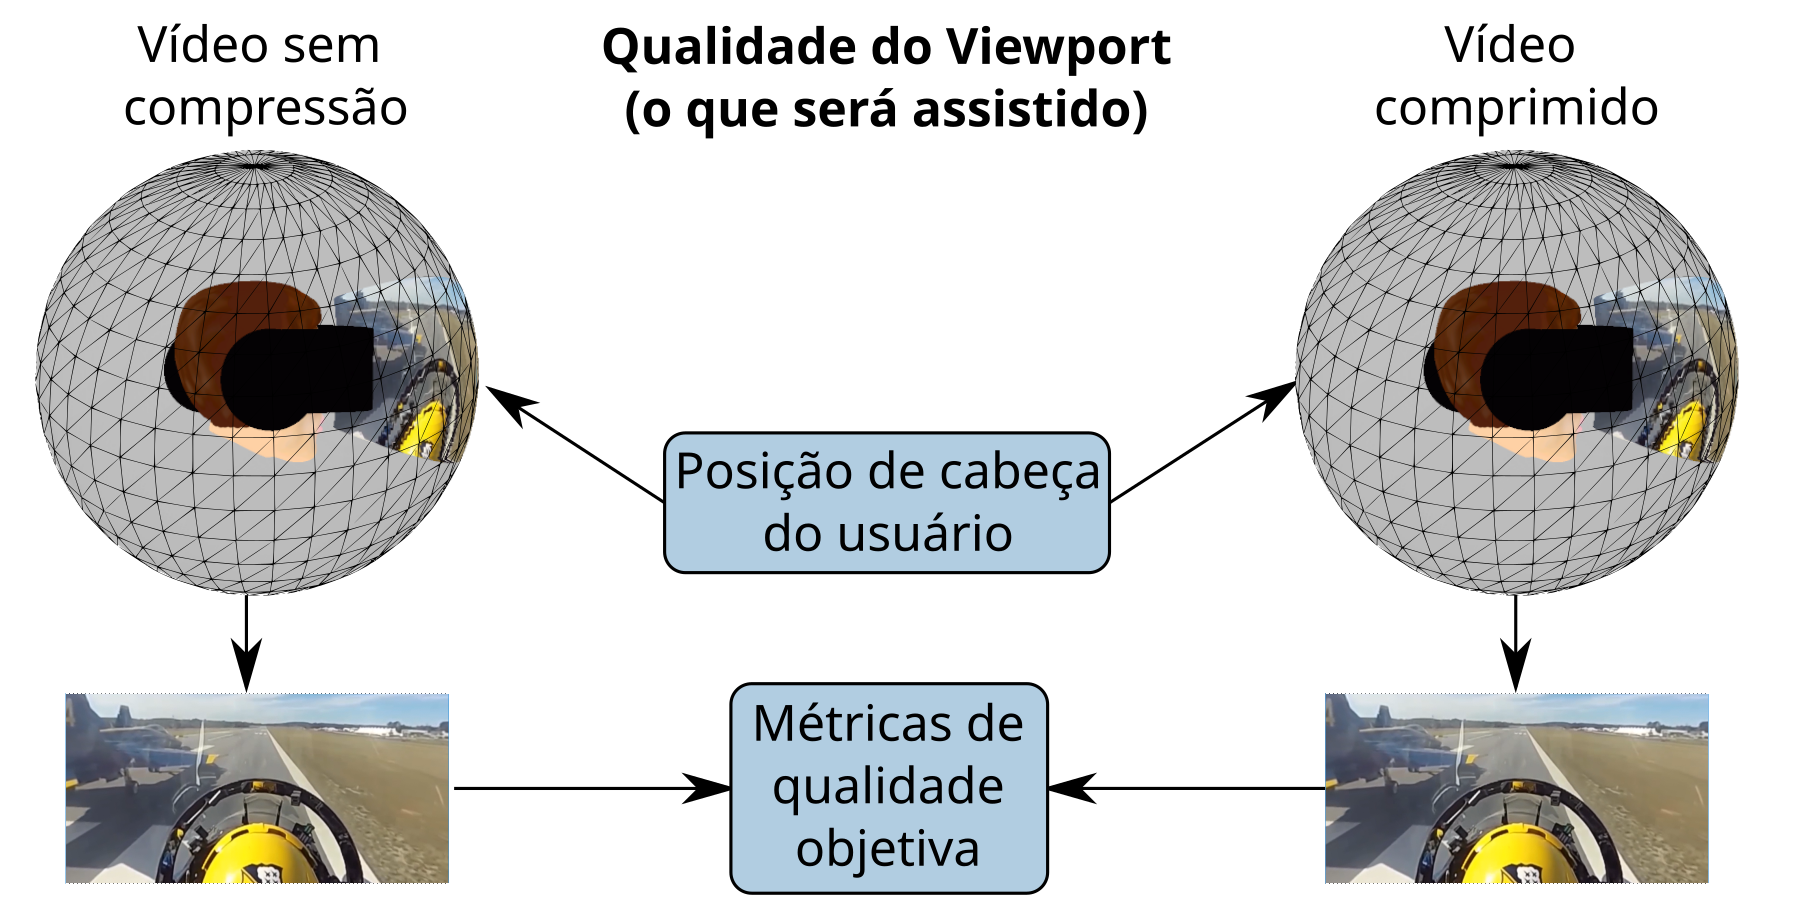
\includegraphics[width=0.8\linewidth]{fig/Project_Quality_Workflow_2.png}
    \caption{Avaliação de qualidade objetiva do viewport.}
    \label{fig:QualityWorkflow}
\end{figure}

Quando o vídeo é segmentado em ladrilhos, é necessário reconstruir a projeção com os ladrilhos que são visualizados durante todo o período de duração de um \textit{chunk}. Como o usuário está movimentando a cabeça, durante um \textit{chunk} os ladrilhos vistos podem se modificar. Para o DASH o \textit{chunk} inteiro precisa estar no \textit{buffer} do cliente para que apenas alguns quadros possam ser decodificados. A aplicação cliente precisa saber de antemão quais ladrilhos serão vistos e então solicitá-los ao servidor. Por exemplo, na figura~\ref{fig:selectTiles} vemos uma projeção equirretangular segmentada em 3x3 ladrilhos. No instante 0 o usuário está visualizando os ladrilhos 3, 4, 6, 7 e 8, porém, devido ao movimento da cabeça, antes de se concluir a reprodução do \textit{chunk}, o usuário passa a ver os ladrilhos 0, 1, 3, 4, 6 e 7. Os ladrilhos 0 e 1 passaram a ser vistos e o ladrilho 8 deixou de ser visto. Os ladrilhos 0 e 1 precisam já ter sido baixados e decodificados para que o usuário veja seu conteúdo nos instantes finais do \textit{chunk}.

\begin{figure}[h]
    \centering
    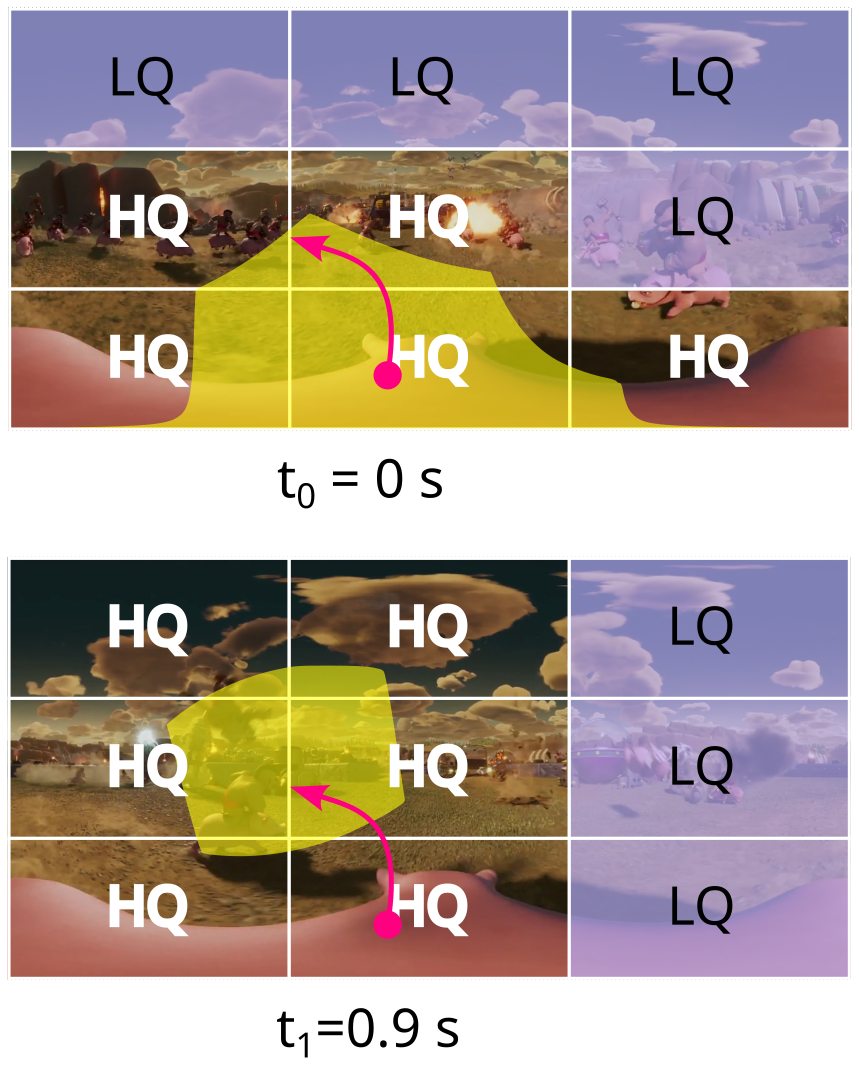
\includegraphics[width=0.5\linewidth]{fig/Streaming of Tiles 2.png}
    \caption{Tiles que deverão ser solicitados ao servidor e que serão assistidos durante um \textit{chunk}.}
    \label{fig:selectTiles}
\end{figure}

Em um cenário com decodificadores operando em paralelo o tempo para a decodificação dos chunks do viewport será igual ao maior tempo de decodificação entre todos os tiles selecionados. Porém, em um ambiente com threads simples, o tempo de decodificação será igual a soma de todos os tempos de decodificação. A taxa de bits necessária para a reprodução do viewport será igual soma de todos os ladrilhos que foram visualizados durante a duração de um chunk.

\subsection{Qualidade para o servidor}

Por outro lado, para sistemas de transmissão adaptativos como o MPEG DASH, a qualidade do vídeo codificado está diretamente correlacionada com sua taxa de bits. Esta correlação baseia-se no pressuposto de que uma taxa de bits mais elevada corresponde a uma melhor qualidade. A lógica por trás dessa relação reside no fato de que a qualidade medida, normalmente avaliada usando métricas como PSNR ou MSE, quantifica o erro induzido pela quantização no processo de compressão com perdas. Neste contexto, o aumento da quantização leva a uma perda de detalhes e a uma maior compressão, reduzindo a qualidade e também a taxa de bits.

No entanto, é importante notar que as métricas SSIM e PSNR podem não ser adequadas para avaliar diretamente a qualidade da projeção, especialmente considerando as distorções introduzidas durante o processo de projeção. Consequentemente, métricas de qualidade esféricas foram desenvolvidas para avaliar o nível objetivo de qualidade de uma projeção. A parte superior da Figura \ref{fig:QualityDiagram} ilustra como a “qualidade objetiva da projeção” deve ser medida. Métricas de qualidade devem ser aplicadas entre a projeção antes da codificação (vídeo de referência) e a projeção decodificada após a compressão (vídeo degradado).

\begin{figure}[htb]
    \centering
    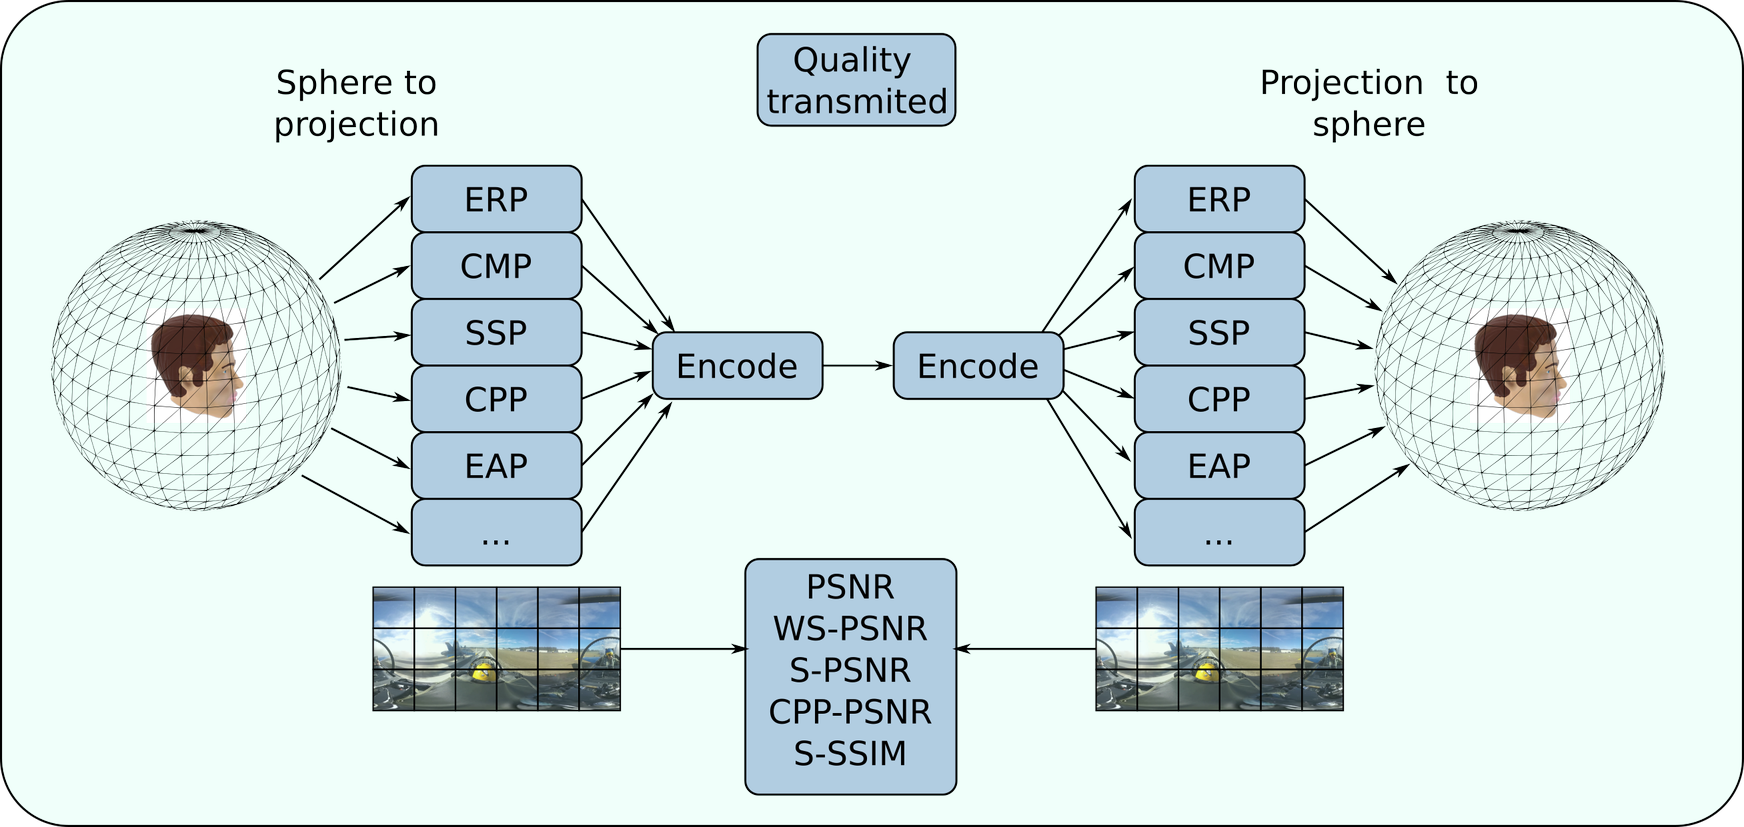
\includegraphics[width=0.7\linewidth]{fig/diagrama e qualidade 1.png}
    \caption{Avaliação de qualidade objetiva da projeção.}
    \label{fig:QualityDiagram}
\end{figure}

Conseguir um vídeo codificado de qualidade alta requer minimizar as perdas a um nível que não seja perceptível o suficiente para causar desconforto. A qualidade objetiva da projeção é definida especificamente como a disparidade entre o vídeo codificado e o vídeo de referência da perspectiva da projeção. Consequentemente, a qualidade objectiva da projeção de vídeo difere da qualidade objetiva da janela de visualização. O que os algoritmos convencionais de taxa de bits adaptativa (ABR) podem considerar satisfatório no domínio de codificação/transmissão pode não estar necessariamente alinhado com a qualidade ideal no domínio da esfera.

Para formular um algoritmo eficaz de adaptação de taxa de bits (ABR) adaptado para streaming de vídeo em 360°, é necessário um estudo aprofundado para compreender a relação entre a qualidade da janela de visualização e a qualidade da projeção. Esse mapeamento torna-se crucial no processo de tomada de decisão para troca de qualidade, reconhecendo que o usuário e o algoritmo ABR operam em planos distintos~\cite{tran2017, Xu2020}.

\subsubsection{MSE/PSNR}

PSNR, ou \textit{Peak Signal-to-Noise Ratio}, e o MSE (\textit{Mean Squared Error}) são métricas amplamente utilizada para avaliar a qualidade de imagens e vídeos reconstruídos ou compactados. Quantifica a relação entre a potência máxima possível de um sinal (neste contexto, uma imagem ou vídeo) e a potência do ruído corruptor que impacta a qualidade do sinal. As duas métricas se relacionam através da seguinte fórmula:

\begin{align}
    \label{MSE}
    MSE&= \frac{1}{M\times N}\sum^{M-1}_{i=0}\sum^{N-1}_{j=0} \left(y(i,j) - y'(i,j)\right)^2 \\
    \label{PSNR}
    PSNR&=10 \times \log_{10}\left(\frac{MAX^2_I}{MSE}\right)
\end{align}

Primeiro, o MSE é calculado para todos os quadros do vídeo e, no final da reprodução, a média do MSE é usado para calcular o PSNR (\textit{Peak Signal-to-Noise Ratio}). Para um vídeo segmentado em ladrilhos, considere que $L_{quadro} $ é a lista de quadros tocados pelo viewport ao longo da reprodução do vídeo e $MSE_{frame}(i)$ é o MSE de um quadro. A qualidade de uma seção de vídeo assistido pelo usuário, é definida pelo PSNR utilizando a média do MSE de todos quadros que aparecerem no viewport, como mostra a equação~\ref{eq:agerage_MSE}.

\begin{equation}
    \bar{MSE} = \sum^{N_{frames}}_{i=0} \dfrac{MSE_{frame}(i)}{N_{frames}}
    \label{eq:agerage_MSE}
\end{equation}

\subsubsection{S-MSE/S-PSNR}

O S-PSNR emprega uma lista de 655.362 pontos equidistantes na esfera para identificar os pixels correspondentes na projeção original e na projeção degradada para em seguida calcular o MSE para todos estes pontos. Este processo é ilustrado na Figura~\ref{fig:spsnr}. Encontra-se o ponto na projeção correspondente ao ponto da esfera e então calcula-se o erro. Desta forma é possível comparar duas projeções diferentes. Apesar desta métrica se preocupar em uniformizar as amostras no domínio da esfera, onde o usuário realmente interage, quanto maior a resolução da projeção, mais pixels serão desprezados no cálculo da métrica.

\begin{figure}[h]
     \centering
     \subfigure[O S-PSNR busca os pixels na projeção de referência ``R'' e a projeção degradada ``T'' correspondentes aos pontos ``S'' pré-definidos e equidistantes na esfera.\label{fig:spsnr}]{
        \quad
        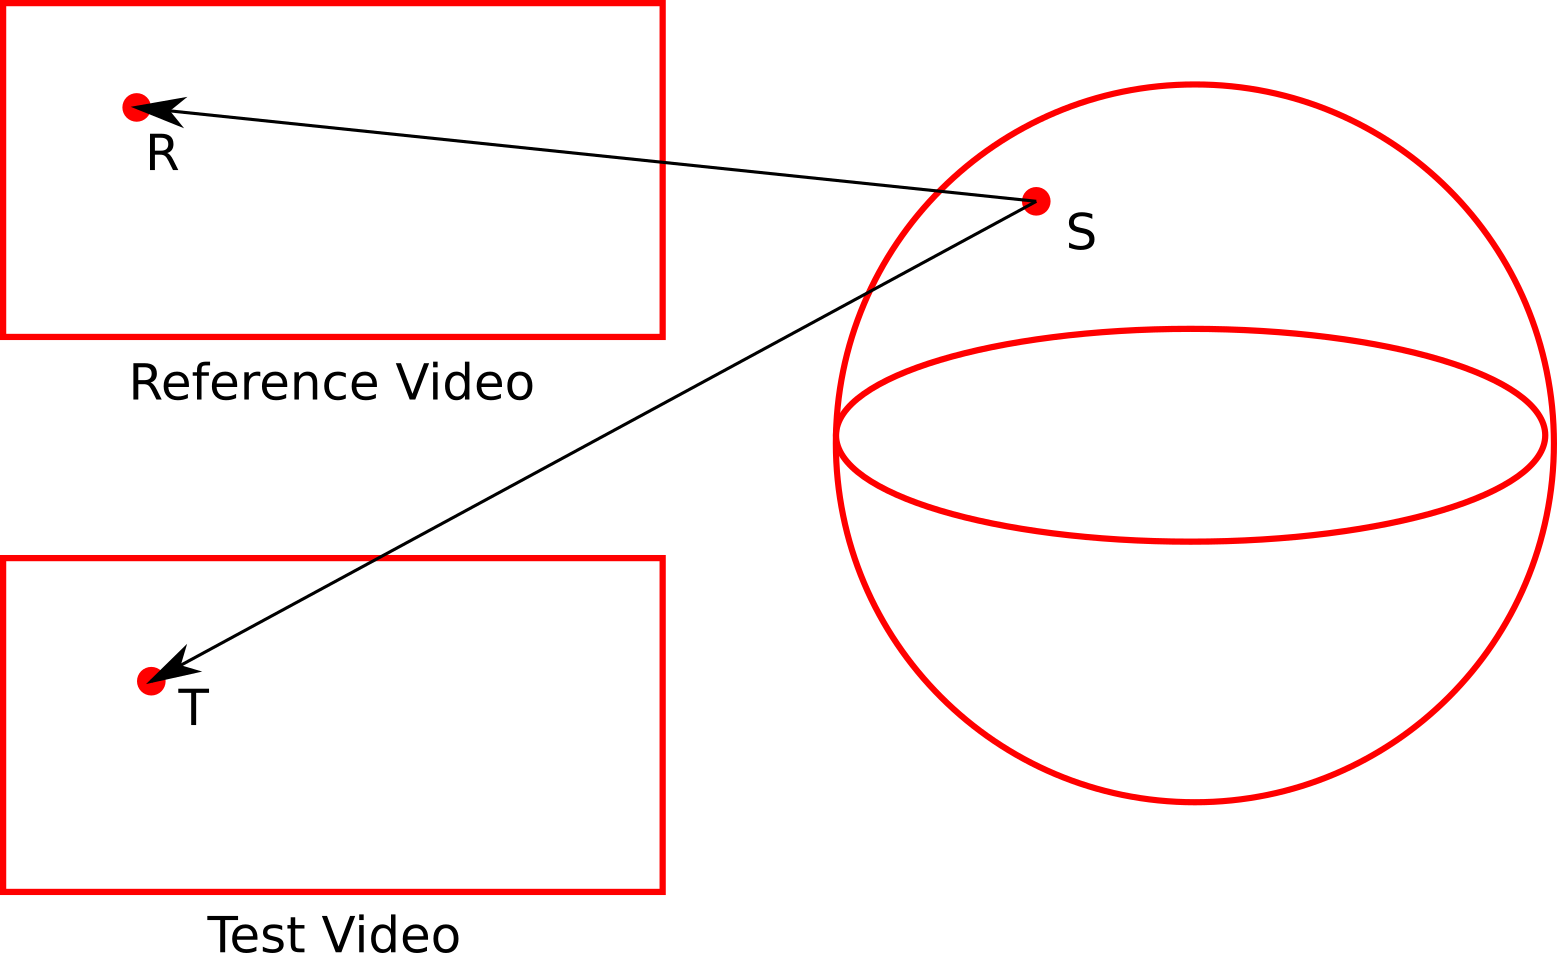
\includegraphics[width=0.4\linewidth]{fig/diag_spsnr.png}
        \quad
     }
     \quad
     \subfigure[Mapa de pesos para a projeção Equirretangular e Cubemap usado pela métrica WS-MSE\label{fig:wspsnr}]{
        \quad\quad
        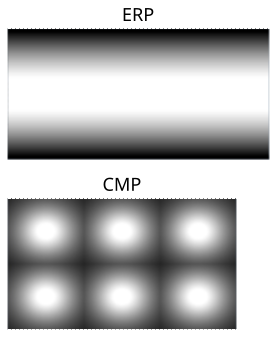
\includegraphics[width=0.25\linewidth]{fig/ws-psnr.png}
        \quad\quad
     }     
\end{figure}

\subsubsection{WS-MSE/WS-PSNR}

O WS-MSE e o WS-PSNR incorporam pesos para cada pixel da projeção ao calcular MSE, conforme expresso nas Equações \ref{eq:WMSE} e \ref{eq:WS-PSNR}. Considerando uma projeção com resolução MxN, o WS-MSE primeiro calcula a média ponderada do quadrado das diferenças dos pixels y e y' na posição (i,j) para todos os pixels de cada quadro. O cálculo do WS-PSNR só é aplicado sobre a média do WS-MSE de todos os quadros.

\begin{align}
   \label{eq:WMSE}
    MSE&= \frac{\sum^{M-1}_{i=0}\sum^{N-1}_{j=0} \left(y(i,j) - y'(i,j)\right)^2 \times w(i,j)}{\sum^{M-1}_{i=0} \sum^{N-1}_{j=0} w(i,j)}\\[12pt]
    \label{eq:WS-PSNR}
    WS\mbox{-}PSNR&=10 \times \log_{10}\left(\frac{MAX^2_I}{MSE}\right)
\end{align}

Os pesos de cada pixel dependem da sua posição na projeção e do tipo de projeção. Projeções como ERP esticam mais os polos enquanto a projeção Cubemap distribui as faces na imagem de forma arbitrária. As equações \ref{eq:w_wpsnr1} e \ref{eq:w_wpsnr2} delineiam os pesos para as projeções equirretangular (ERP) e cubemap (CMP). No caso de uma projeção Cubemap, considera-se que todas as faces do cubo são quadradas e possuem resolução $A \times A$. O resultado pode ser visto na figura~\ref{fig:wspsnr}

\begin{align}
    \label{eq:w_wpsnr1}
    w_{ERP}(i,j)&=cos\left(\frac{(j+0.5-N/2)\pi}{N}\right) \\
    \label{eq:w_wpsnr2}
    w_{CMP}(i,j)&=\left(1 + \frac{d^2(i,j)}{r^2}\right)^{\frac{-3}{2}} \\
    d^2(i, j)&=(i+0.5-\dfrac{A}{2})^2 +(j+0.5-\dfrac{A}{2})^2
\end{align}

\subsection{Estatísticas}

Determinar as estatísticas das métricas é muito importante afim de entender seu comportamento e distribuição ao longo da reprodução para diferentes tipos de conteúdos. A distribuição das métricas de tempo de decodificação, taxa de bits e qualidade objetiva foram analisadas considerando que as distribuições são positivas e contínuas, descartando distribuições discretas e distribuições sobre a reta real. Considerando também as distribuições disponíveis nos pacotes estatísticos mais comuns, como SciPy e Matlab, as distribuições analisadas são: Burr Tipo XII , Birnbaum-Saunders, Gamma, Inversa Gaussiana, Rayleigh, Log Normal, Generalized Pareto, Pareto, Half-Normal, e Exponencial. O processo de ajuste mais comum se baseia na estimação dos parâmetros por máxima verossimilhança e para a avaliação das distribuições foi utiliza o erro quadrático médio (RMSE).

A correlação entre as métricas é feita entre todos os chunks de cada ladrilho. Como a correlação mede a dependência entre duas variáveis e as métricas variam de forma diferente para cada tipo de ladrilhamento e para cada qualidade de codificação, a correlação deve ser medida considerando apenas as ladrilhos de uma mesma qualidade e de uma mesma região de cada vídeo. Assim, as métricas de 60 chunks para cada ladrilho, para cada qualidade e para cada vídeo puderam ser correlacionada. Por fim a média de todas as correções são consideradas ao se comparar diferentes cenários.
